\documentclass{controle}
\usepackage{main}

\title{Variables aléatoires : Entraînement}
\author{TSTMG1}
\date{Chapitre 5 : Variables aléatoires}

\begin{document}
\maketitle

\begin{questions}
\question Construire le triangle de pascal pour calculer les coefficients binomiaux $\binom{n}{k}$ pour $n \leq 8$. En déduire la valeur des coefficients suivants :
\begin{parts}
\part $\binom{6}{2}$
\part $\binom{7}{4}$
\part $\binom{8}{5}$
\end{parts}
\vspace*{1cm}
\question On joue au jeu suivant : dans une urne opaque, on installe $2$ boules rouges numérotées $2$; $3$ boules bleues numérotées $-1$ et une boule noire numérotée $\times 2$. On tire au hasard deux boules simultanément dans cette urne, et on gagne une somme d'argent correspondant à la somme des deux tirages. Si on a tiré la boule noire, on multiplie le gain (ou la perte) par deux.

On note $X$ le gain en euros suite à ce jeu.

\begin{parts}
\part Compléter l'arbre de probabilités ci-dessous.

%:-+-+-+- Engendré par : http://math.et.info.free.fr/TikZ/Arbre/
\begin{center}
% Racine à Gauche, développement vers la droite
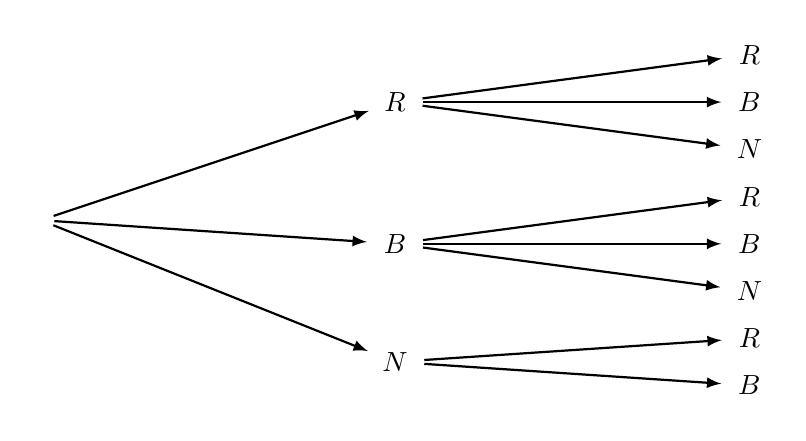
\begin{tikzpicture}[xscale=1.5,yscale=0.3]
% Styles (MODIFIABLES)
\tikzstyle{fleche}=[->,>=latex,thick]
\tikzstyle{noeud}=[circle]
\tikzstyle{feuille}=[circle]
% Dimensions (MODIFIABLES)
\def\DistanceInterNiveaux{3}
\def\DistanceInterFeuilles{2}
% Dimensions calculées (NON MODIFIABLES)
\def\NiveauA{(0)*\DistanceInterNiveaux}
\def\NiveauB{(1)*\DistanceInterNiveaux}
\def\NiveauC{(2)*\DistanceInterNiveaux}
\def\InterFeuilles{(-1)*\DistanceInterFeuilles}
% Noeuds (MODIFIABLES : Styles et Coefficients d'InterFeuilles)
\node[noeud] (R) at ({\NiveauA},{(3.5)*\InterFeuilles}) {$ $};
\node[noeud] (Ra) at ({\NiveauB},{(1)*\InterFeuilles}) {$R$};
\node[feuille] (Raa) at ({\NiveauC},{(0)*\InterFeuilles}) {$R$};
\node[feuille] (Rab) at ({\NiveauC},{(1)*\InterFeuilles}) {$B$};
\node[feuille] (Rac) at ({\NiveauC},{(2)*\InterFeuilles}) {$N$};
\node[noeud] (Rb) at ({\NiveauB},{(4)*\InterFeuilles}) {$B$};
\node[feuille] (Rba) at ({\NiveauC},{(3)*\InterFeuilles}) {$R$};
\node[feuille] (Rbb) at ({\NiveauC},{(4)*\InterFeuilles}) {$B$};
\node[feuille] (Rbc) at ({\NiveauC},{(5)*\InterFeuilles}) {$N$};
\node[noeud] (Rc) at ({\NiveauB},{(6.5)*\InterFeuilles}) {$N$};
\node[feuille] (Rca) at ({\NiveauC},{(6)*\InterFeuilles}) {$R$};
\node[feuille] (Rcb) at ({\NiveauC},{(7)*\InterFeuilles}) {$B$};
% Arcs (MODIFIABLES : Styles)
\draw[fleche] (R)--(Ra);
\draw[fleche] (Ra)--(Raa);
\draw[fleche] (Ra)--(Rab);
\draw[fleche] (Ra)--(Rac);
\draw[fleche] (R)--(Rb);
\draw[fleche] (Rb)--(Rba);
\draw[fleche] (Rb)--(Rbb);
\draw[fleche] (Rb)--(Rbc);
\draw[fleche] (R)--(Rc);
\draw[fleche] (Rc)--(Rca);
\draw[fleche] (Rc)--(Rcb);
\end{tikzpicture}
\end{center}
%:-+-+-+-+- Fin

\part Quelles sont les différents gains possibles ?
\part En déduire la loi de $X$.
\part Calculer l'espérance de $X$.
\part Le jeu est-il rentable ?
\end{parts}
\vspace*{1cm}
\question Un entreprise produit des pièces pour des pompes à chaleur. Elle constate que sur un grand nombre de pièces produites, $4\%$ d'entre elles ont un défaut.

On tire $8$ pièces au hasard dans la production, et on note $X$ le nombre de pièces avec un défaut dans le tirage.
\begin{parts}
\part Justifier que $X$ suit une loi binomiale dont on précisera les paramètres.
\part Quelle est la probabilité que le nombre de pièces avec un défaut dans le tirage soit $2$ ?
\part Quelle est la probabilité que le nombre de pièces avec un défaut dans le tirage soit supérieur ou égal à $7$ ?
\part Quelle est l'espérance de $X$ ? 
\end{parts}
\end{questions}
\end{document}